\section{編輯器介紹}

對於一個引擎而言,除了內部的程式操作外,亦需要一個面對於使用者的GUI來進行操作。
其作用為讓開發者在進行開發時,可以簡化其操作步驟並方便的進行創作,透過對引擎可視化工具的操作來建置與修改遊戲內的場景與物體。

\subsection{版面配置與操作介紹}

打開 RishEditor (RishEngine 的編輯器)可以看到版面就跟市面上常見的編輯器雷同。大致上可以分成四個區塊:工具欄、主要編輯視窗、遊戲物件(Entity)編輯視窗、Log。

\begin{figure}[h]
    \begin{center}
    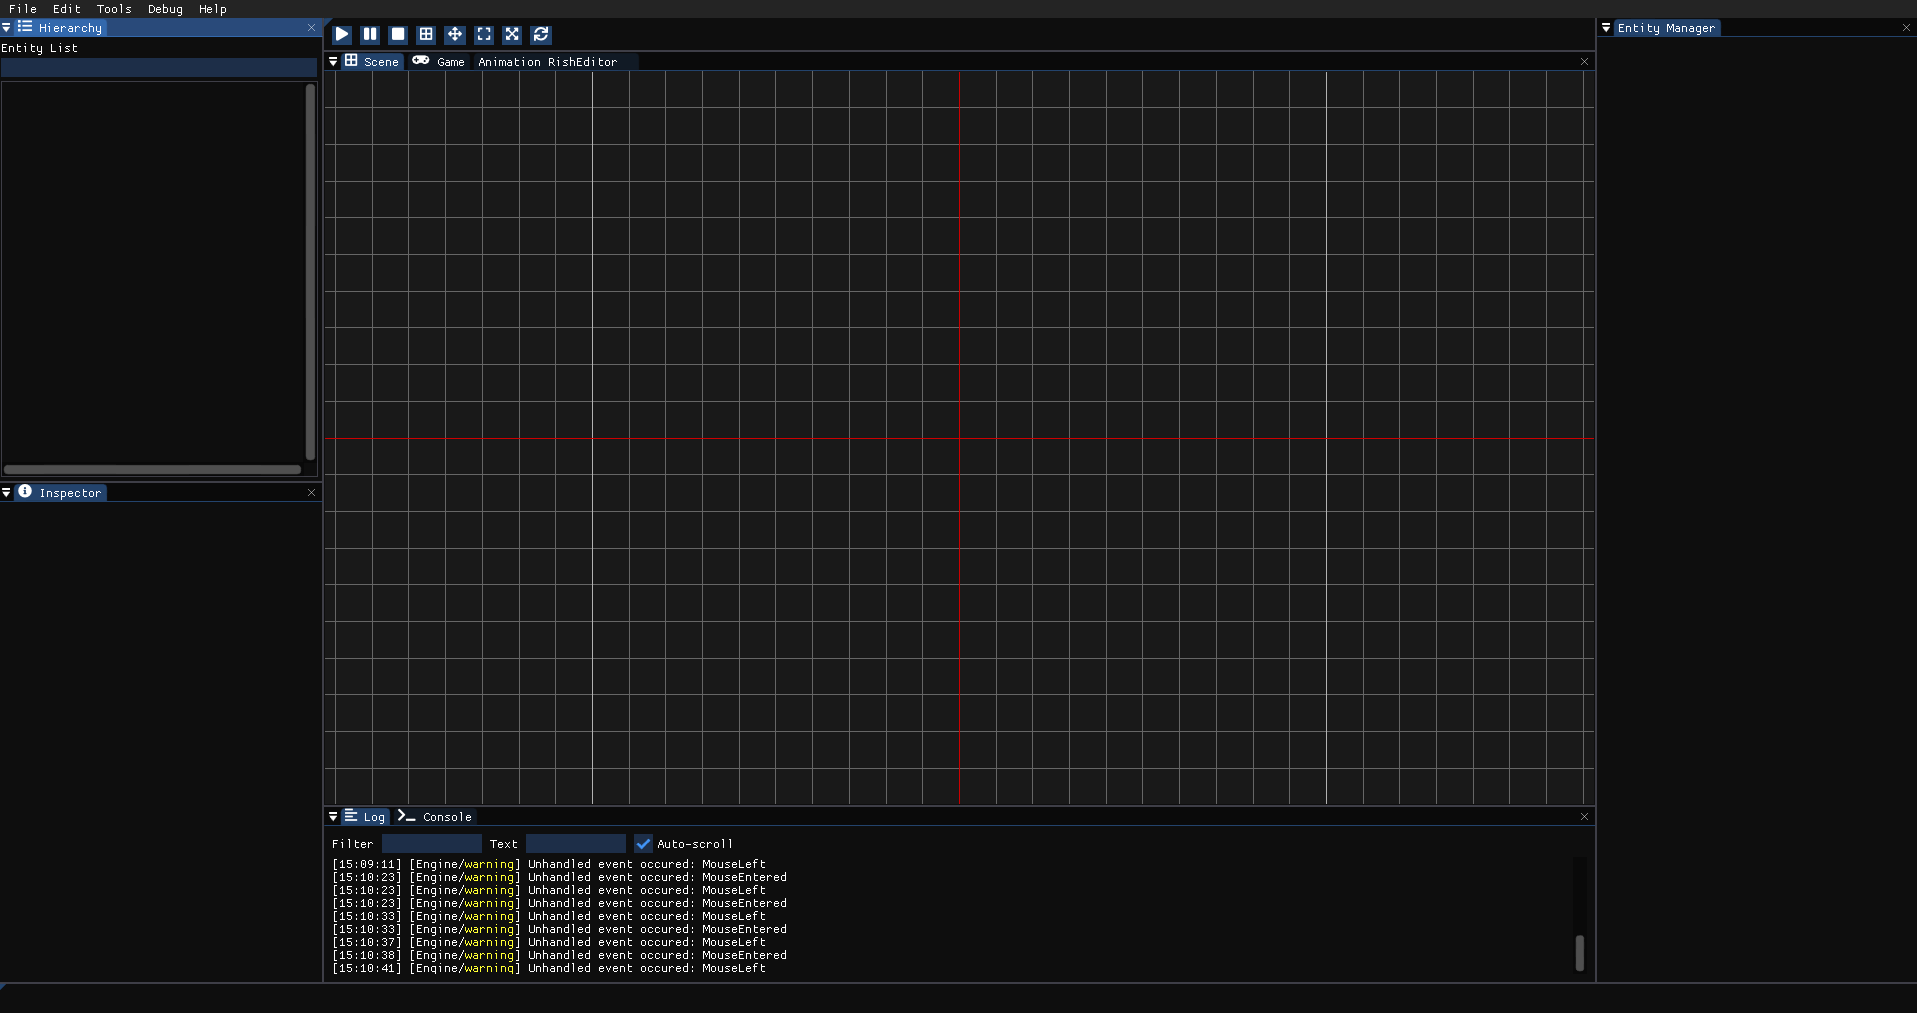
\includegraphics[width=\textwidth]{./resources/editor/all.png}
    \end{center}
\caption{編輯器整體介面}
\label{fig:editor_all}
\end{figure}

\subsubsection{主選單 MenuBar}

\begin{itemize}
\item{File}
    \SubItem{新增、開啟、儲存目前正在編輯的遊戲場景(Scene)}
\item{Edit}
    \SubItem{對遊戲物件 (Entity) 之操作: 複製、貼上、刪除}
\item{Tools}
    \SubItem{對 Editor 進行設定}
\item{Help}
    \SubItem{引擎介紹與製作團隊說明}
\end{itemize}

% https://tex.stackexchange.com/questions/126818/minipage-with-four-figures-avoiding-too-much-whitespace
\begin{figure}[h]
    \begin{subfigure}[b]{0.5\linewidth}
        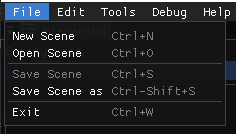
\includegraphics[width=\linewidth]{./resources/editor/a.png} 
        \caption{File 選單}
    \end{subfigure}
    \begin{subfigure}[b]{0.5\linewidth}
        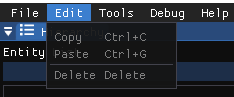
\includegraphics[width=\linewidth]{./resources/editor/b.png}
        \caption{Edit 選單}
    \end{subfigure}
    \begin{subfigure}[b]{0.5\linewidth}
        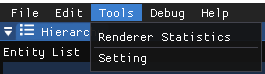
\includegraphics[width=\linewidth]{./resources/editor/c.png}
        \caption{Tools 選單}
    \end{subfigure}
    \begin{subfigure}[b]{0.5\linewidth}
        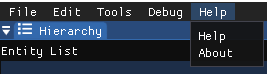
\includegraphics[width=\linewidth]{./resources/editor/d.png}
        \caption{Help 選單}
    \end{subfigure}
\caption{主選單介面}
\label{fig:MenuBar}
\end{figure}

%%%%%%%%%%%%%%%%%%%%%%%%%%%%%%%%%%%%%%%%%%%%%%%%%%%%%%%%%%%%%%%%%%%%%%%%
\subsubsection{引擎實體列表 Hierarchy}

補圖

\begin{itemize}
\item{主要為顯示場景中的Entity清單,並可對其進行操作}
    \SubItem{滑鼠左鍵點擊選取Entity,按住Ctrl、Shift可進行多選}
    \SubItem{滑鼠右鍵開啟選單對Entity進行進一步的操作}
        \SubSubItem{新增、複製、貼上、刪除Entity}
        \SubSubItem{將多個Entity設定為Group一起操作}
    \SubItem{可將單一Entity用滑鼠拖曳進其他Entity中,使其成為Group}
\end{itemize}

%%%%%%%%%%%%%%%%%%%%%%%%%%%%%%%%%%%%%%%%%%%%%%%%%%%%%%%%%%%%%%%%%%%%%%%%
\subsubsection{引擎實體檢視 Inspector}

補圖

\begin{itemize}
\item{顯示單一Entity所擁有的Component並加以操作}
    \SubItem{新增、刪除、修改數值}
\item{Component的操作介面}
    \SubItem{新增、刪除、修改數值}

\end{itemize}


%%%%%%%%%%%%%%%%%%%%%%%%%%%%%%%%%%%%%%%%%%%%%%%%%%%%%%%%%%%%%%%%%%%%%%%%
\subsubsection{工具欄 ToolBar}

\begin{figure}[h]
    \begin{center}
    
\includegraphics[width=0.6\textwidth]{./resources/editor/toolbar.png}
    \end{center}
\caption{工具欄介面}
\label{fig:editor_all}
\end{figure}

\begin{itemize}
\item{Start}
    \SubItem{將場景切換到Game介面,並開始進行測試}
\item{Pause}
    \SubItem{將Game介面的動作暫停}
\item{Stop}
    \SubItem{結束測試返回Scene介面}
\item{Grid}
    \SubItem{顯示/隱藏世界坐標軸}
\item{Move}
    \SubItem{將Gizmo的模式切換為MoveMode}
\item{Zoom}
    \SubItem{將Gizmo的模式切換為ZoomMode}
\item{Scale}
    \SubItem{將Gizmo的模式切換為ScaleMode}
\item{Rotate}
    \SubItem{將Gizmo的模式切換為RotateMode}
\end{itemize}

%%%%%%%%%%%%%%%%%%%%%%%%%%%%%%%%%%%%%%%%%%%%%%%%%%%%%%%%%%%%%%%%%%%%%%%%
\subsubsection{場景視窗 Scene View}

補圖

\begin{itemize}
\item{顯示所創建的Entity}
    \SubItem{滑鼠左鍵點選或圈選Entity,並根據Gizmo的模式對其進行相對應的操作}
    \SubItem{滑鼠右鍵移動視角}
    \SubItem{滑鼠滾輪進行縮放}
    \SubItem{使用快捷鍵對 Entity 進行操作}
        \SubSubItem{`Ctrl+A` 全選}
        \SubSubItem{`Ctrl+C` 複製}
        \SubSubItem{`Ctrl+V` 貼上}
        \SubSubItem{`Ctrl+G` 將選取的Entity放到一Group中}
        \SubSubItem{`Delete` 將選取的Entity刪除}
        \SubSubItem{`Esc` 取消選取Entity }
\end{itemize}

\subsubsection{Gizmo}

補說明

可讓使用者直觀的對 Entity 的大小與位置進行調整

\begin{figure}[h]
    \begin{subfigure}[b]{0.5\linewidth}
        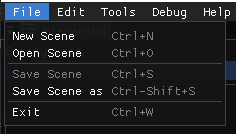
\includegraphics[width=\linewidth]{./resources/editor/a.png} 
        \caption{移動模式}
    \end{subfigure}
    \begin{subfigure}[b]{0.5\linewidth}
        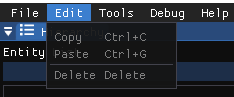
\includegraphics[width=\linewidth]{./resources/editor/b.png}
        \caption{拉伸模式}
    \end{subfigure}
    \begin{subfigure}[b]{0.5\linewidth}
        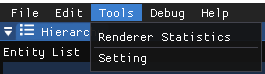
\includegraphics[width=\linewidth]{./resources/editor/c.png}
        \caption{縮放模式}
    \end{subfigure}
    \begin{subfigure}[b]{0.5\linewidth}
        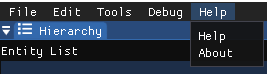
\includegraphics[width=\linewidth]{./resources/editor/d.png}
        \caption{旋轉模式}
    \end{subfigure}
\caption{Gizmo 的不同模式}
\label{fig:MenuBar}
\end{figure}

\begin{itemize}
\item{移動}
    \SubItem{滑鼠按壓中間黃色區塊拖曳Entity移動位置}
    \SubItem{按壓藍色箭頭限定水平移動}
    \SubItem{按壓紅色箭頭限定垂直移動}
\item{拉伸}
    \SubItem{在Entity上下左右與角落處共八個區塊}
    \SubItem{按壓並拖曳各個區塊皆可改變 Entity 的大小}
\item{縮放}
    \SubItem{對於Entity的長與寬從中心延伸出紅線與藍線}
    \SubItem{在尾端有黃色區塊可按壓拖曳改變Entity的長與寬}
\item{旋轉}
    \SubItem{可將Entity進行旋轉,會有一紅線表示現Entity的旋轉角度}
\end{itemize}

%%%%%%%%%%%%%%%%%%%%%%%%%%%%%%%%%%%%%%%%%%%%%%%%%%%%%%%%%%%%%%%%%%%%%%%%
\subsubsection{遊戲視窗 Game View}

補圖

在測試期間將會顯示標示為primary的CameraComponent的視角並運行各個Component的動作

%%%%%%%%%%%%%%%%%%%%%%%%%%%%%%%%%%%%%%%%%%%%%%%%%%%%%%%%%%%%%%%%%%%%%%%%
\subsubsection{除錯訊息視窗 Log}

\begin{figure}[h]
    \begin{center}
    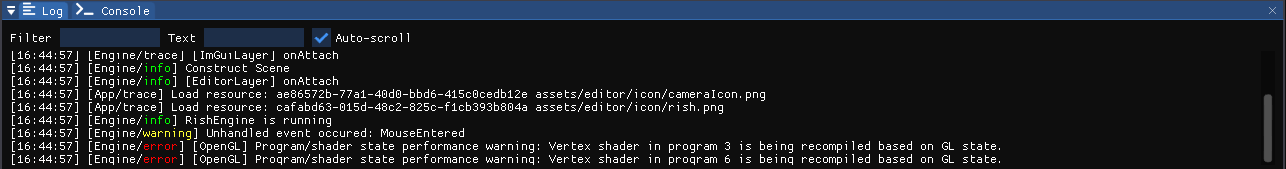
\includegraphics[width=\textwidth]{./resources/editor/logger.png}
    \end{center}
\caption{工具欄介面}
\end{figure}

\begin{itemize}
\item{顯示開發人員輸出或引擎輸出之訊息,並將其分級顯示}
    \SubItem{依照錯誤級別分成: TRACE, INFO, WARN, ERROR, CRITICAL}
\item{可對 Log 進行過濾,方便遊戲開發者在眾多訊息中定位}
\end{itemize}

%%%%%%%%%%%%%%%%%%%%%%%%%%%%%%%%%%%%%%%%%%%%%%%%%%%%%%%%%%%%%%%%%%%%%%%%
\subsubsection{Editor 訊息視窗 Status}

補圖

顯示目前Editor的狀態


%%%%%%%%%%%%%%%%%%%%%%%%%%%%%%%%%%%%%%%%%%%%%%%%%%%%%%%%%%%%%%%%%%%%%%%%%%%%%%%%%%%%%%%%%%%%%%%%%%%%%%%%%%%%%%%%%%%%%%%%%%%%%%%%%%%%%%%%%%%%%%%%
\subsection{架構}

\begin{figure}[t]
    \begin{center}
    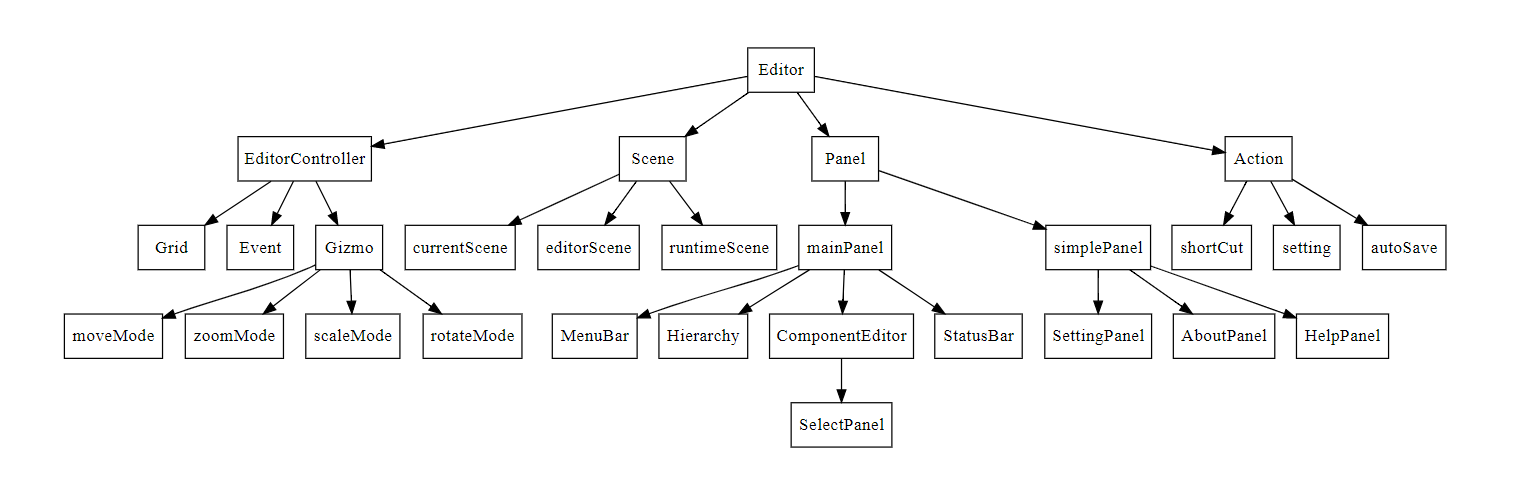
\includegraphics[width=\textwidth]{./resources/editor/arch.png}
    \end{center}
\caption{Editor 架構}
\label{fig:editor_arch}
\end{figure}

\begin{itemize}
\item Editor
    \SubItem{在Editor底下利用EditorController管理著 Scene, Panel, Action}
    \SubItem{Scene 為遊戲世界的畫面管理}
    \SubItem{Panel 為 Editor 的介面管理}
    \SubItem{Action 為 Editor 中的各式操作}
\end{itemize}

\begin{itemize}
\item{EditorController}
    \SubItem{Grid}
    \SubItem{Event}
        \SubSubItem{接收滑鼠與鍵盤的操作}
    \SubItem{Gizmo}
        \SubSubItem{移動模式}
            \SubSubSubItem{根據滑鼠點擊的位置來決定Entity移動時的權重}
            \SubSubSubItem{根據滑鼠拖拉的距離去乘上權重來改變Entity的位置}
        \SubSubItem{拉伸模式}
            \SubSubSubItem{根據滑鼠點擊的位置來決定Entity移動時的權重與其大小的權重}
            \SubSubSubItem{根據滑鼠拖拉的距離去分別乘上各自的權重來改變其位置與大小}
        \SubSubItem{縮放模式}
            \SubSubSubItem{根據滑鼠點擊的位置來決定要改變Entity的長或寬}
            \SubSubSubItem{根據滑鼠拖拉的向量與要改變的Entity方向去計算其投影向量}
            \SubSubSubItem{根據該投影向量來計算需增加的長或寬}
        \SubSubItem{旋轉模式}
            \SubSubSubItem{根據滑鼠拖拉時的起始點與最終點分別與Entity的中心點作為向量}
            \SubSubSubItem{計算二向量的夾角來改變Entity的rotate}
\end{itemize}

\begin{itemize}
\item{Scene}
    \SubItem{currentScene}
    \SubItem{editorScene}
        \SubSubItem{在Editor模式下所使用的Scene}
    \SubItem{runtimeScene}
        \SubSubItem{在遊戲模式下所使用的Scene}
\end{itemize}

\begin{itemize}
\item{Panel}
    \SubItem{mainPanel 主要顯示的視窗}
        \SubSubItem{MenuBar}
            \SubSubSubItem{管理simplePanel以及與Editor相關之API}
        \SubSubItem{Hierarchy}
            \SubSubSubItem{從currentScene中拿到其所有的Entity並顯示其tag}
            \SubSubSubItem{標記部分Entity為選取狀態並對其進行操作}
        \SubSubItem{ComponentEditor}
            \SubSubSubItem{對於所選取之Entity的Component進行操作}
            \SubSubSubItem{使用各個Component的API來進行操作}
            \SubSubSubItem{選取視窗顯示所有可新增的Component,點選後將其新增到Entity上}
        \SubSubItem{StatusBar}
            \SubSubSubItem{接收EditorController發送的訊息並顯示}
    \SubItem{simplePanel 簡易的彈跳式視窗}
        \SubSubItem{SettingPanel}
            \SubSubSubItem{讀取並修改Editor的設定檔}
        \SubSubItem{HelpPanel}
        \SubSubItem{AboutPanel}
\end{itemize}

\begin{itemize}
\item{Action}
    \SubItem{shortCut}
        \SubSubItem{設定各個快捷鍵的操控}
    \SubItem{setting}
        \SubSubItem{設定Editor}
    \SubItem{autoSave}
        \SubSubItem{每過一段時間自動將Editor的Scene儲存起來}
\end{itemize}

\subsection{未來展望}

寫太少

\begin{itemize}
\item{Undo \& Redo System}
    \SubItem{讓使用者可以回復其所做的上一步操作}
\item{支援3D顯示與操作}
    \SubItem{在引擎的各項功能提供3D操作後,讓Editor亦可供其顯示與操作}
\end{itemize}

